\subsection*{A14.8}
\subsubsection*{(a)}
The problem can be formed into the following optimization problem:
\begin{align*}
&minimize \qquad \sum_{K}||f_k(t)||_2 \\
&subject \ to \qquad   ||f_k(t)||_2 \leq \text{Fmax} \qquad k =1,...,K\\
&\qquad \qquad \qquad \ \alpha||A^Tp_k(t)||_2 -e_3p_k(t) \leq 0 \\
&\qquad \qquad \qquad \ v_{k+1} =v_k +(h/m)f_k -hge_3 \\
&\qquad \qquad \qquad \ p_{k+1} =p_k + (h/2) (v_k +v_{k+1})\\
&\qquad \qquad \qquad \ v_{des} =p_{des} = 0 \\
&\qquad \qquad \qquad \ p_{init} = p_0 \\
&\qquad \qquad \qquad \ v_{init} = v_0 \\
\end{align*}  
\paragraph{}
Where variable $[f_k(t), p_k(t), v_k(t)]^T \in R^{9\times36}$, and $A = [1\ 1\ 0]^T$. This is a convex optimization problem since the objective function is convex and all constraints are either convex or linear.
\subsubsection*{(b)}
\paragraph{}
We can solve this problem by fixing K to a number starting from 1 and increasing K till we find a solution.
\subsubsection*{(c)}
For (a) $p^{\star} =193$ and for (b) $p^{\star}=25$. Attached are code and figures.
\begin{figure}
	\centering
	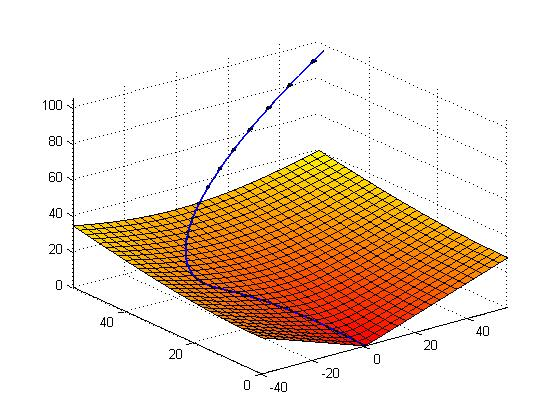
\includegraphics[scale=0.7]{trag}
	\caption{Min Fuel Trajectory}
\end{figure}
\begin{figure}
	\centering
	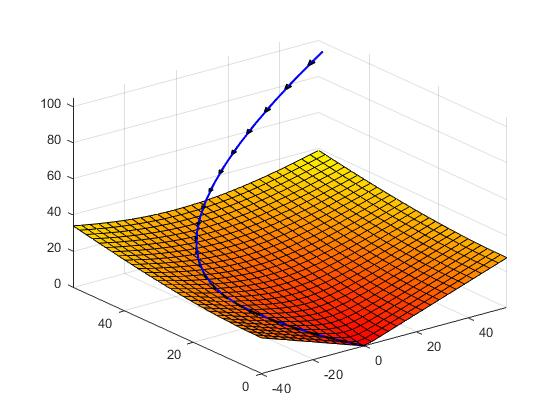
\includegraphics[scale=0.7]{trag2}
	\caption{Min Time Trajectory}
\end{figure}
\paragraph{Min Fuel}
\verbatiminput{sc_ld_main.m}
\paragraph{Min Time}
\verbatiminput{sc_kmin_main.m}